\chapter{تكيفات النبات واللدونة النمطية}\label{ch:b2:plant-plasticity}

ورقتان من البلوطة نفسها: فالمأخوذة من أعلى التاج
صغيرة سميكة جلدية، والمأخوذة من الداخل المظلل أكبر منها
ثلاث مرات ورقيقة كالورق. وبادرة من البلوطة نفسها تحت
مظلة مغلقة تنمو طويلة نحيلة؛ وشقيقتها في فرجة تبقى
قصيرة متينة. ولا فرق من هذين وراثي. فالنبات لا يستطيع أن يمشي
إلى مكان أفضل، فيبني نفسه ليلائم المكان الذي هو فيه: إذ
يستشعر الضوء والجاذبية واللمس والماء والملح والبرد، وينحني
ويثخن ويستطيل ويغلق مسامه أو يقسّي خلاياه
تبعًا لذلك. وهذا الفصل عن تلك اللدونة --- كيف يقرأ النبات
محيطه وماذا يفعل حياله --- وعن
التكيفات الموروثة التي لاءمت بها السلالات نفسها
مع الصحارى والظل والملح والصقيع.

\section{اللدونة وحدودها}

\begin{definition}[اللدونة النمطية ومعيار الاستجابة]\label{def:b2:plant-plasticity:plasticity}
\index{لدونة نمطية}\index{معيار الاستجابة}\index{تأقلم}\index{تكيف}
\emph{اللدونة النمطية} قدرة \omterm{def:b2:meiosis-heredity:vocabulary}{نمط وراثي} واحد على
إنتاج أنماط ظاهرية مختلفة في بيئات مختلفة. و\emph{معيار
الاستجابة} \omterm{def:b2:meiosis-heredity:vocabulary}{لنمط وراثي} هو منحني نمطه الظاهري
بدلالة متغير بيئي --- ثخن الورقة بدلالة الضوء،
وطول الساق بدلالة الحرارة؛ وتختلف الأنماط الوراثية في معاييرها،
والفروق موروثة حتى حين لا تكون اللدونة نفسها
موروثة. و\emph{التأقلم} هو الصورة العكوسة الفيزيولوجية:
ورقة تثخّن بشرتها في أسبوع جاف، وخلية تصنع
مانع تجمد في الخريف. أما \emph{التكيف}، بالمعنى التطوري،
فهو ملاءمة سلالة موروثة لموئلها، منتخبةً على مدى
الأجيال؛ فالصبار متكيف مع الجفاف، والفاصولياء تتأقلم مع
موجة جفاف. والنباتات أشد لدونة من الحيوانات لأنها
معيارية غير محددة (\cref{ch:b2:plant-meristems}): فالورقة
التالية يمكن أن تُبنى على غير ما بُنيت الأخيرة، والحياة الثابتة
تجعل اللدونة الطريقة الوحيدة للحركة.
\end{definition}

\begin{omfigure}
\begin{tikzpicture}
\begin{axis}[
  width=0.72\linewidth, height=5.4cm,
  axis x line=bottom, axis y line=left,
  xmin=0, xmax=100, ymin=0, ymax=1.2,
  xlabel={الضوء (\% من الشمس الكاملة)}, ylabel={ثخن الورقة (نسبيًا)},
  xlabel style={font=\small, at={(axis description cs:0.5,-0.13)}, anchor=north},
  ylabel style={font=\small},
  tick label style={font=\small}, xtick={0,25,50,75,100}, ytick={0,0.5,1},
  legend style={font=\scriptsize, at={(0.97,0.08)}, anchor=south east, draw=none},
  clip=false,
]
\addplot[very thick, omDef, domain=2:100, samples=60] {0.35 + 0.65*(1-exp(-x/30))};
\addlegendentry{النمط الوراثي 1: بلوطة لدنة}
\addplot[very thick, omThm, domain=2:100, samples=60] {0.55 + 0.2*(1-exp(-x/30))};
\addlegendentry{النمط الوراثي 2: أقل لدونة}
\end{axis}
\end{tikzpicture}

{\small معياران للاستجابة. كل \omterm{def:b2:meiosis-heredity:vocabulary}{نمط وراثي} يصنع أوراقًا أثخن في
ضوء أكثر؛ وميل المنحني --- أي اللدونة --- صفة موروثة
بنفسها، والنمطان الوراثيان يختلفان فيها.}
\end{omfigure}

\begin{proposition}[أوراق الشمس وأوراق الظل]\label{prop:b2:plant-plasticity:sunshade}
\index{ورقة شمس}\index{ورقة ظل}
الورقة النامية في شمس كاملة صغيرة سميكة، بطبقتين أو ثلاث
من الخلايا العمادية، وثغور كثيرة، وبشرة سميكة، وتركيز عالٍ
من إنزيم تثبيت الكربون ومعدل أقصى عالٍ من
التركيب الضوئي؛ أما ورقة النبات نفسه النامية في الظل فكبيرة
رقيقة، بطبقة عمادية واحدة، وكلوروفيل أكثر لوحدة
الكتلة، ومعدل تنفس منخفض، ونقطة تعويض ضوئي منخفضة. و
\omterm{prop:b2:plant-plasticity:sunshade}{ورقة الظل} مبنية لحصد كل فوتون بأدنى كلفة، \omterm{prop:b2:plant-plasticity:sunshade}{وورقة
الشمس} لاستعمال فيض منها دون أن تفرط في الحرارة أو تذبل. و
القرار يُتخذ والورقة لا تزال بدائية، من
الضوء --- ولا سيما لونه --- الذي يبلغ البرعم؛
والورقة الناضجة لا تستطيع إعادة بناء نفسها، ولهذا يحترق النبات المنقول من
الظل إلى الشمس حتى يصنع أوراقًا جديدة.
\end{proposition}

\begin{omfigure}
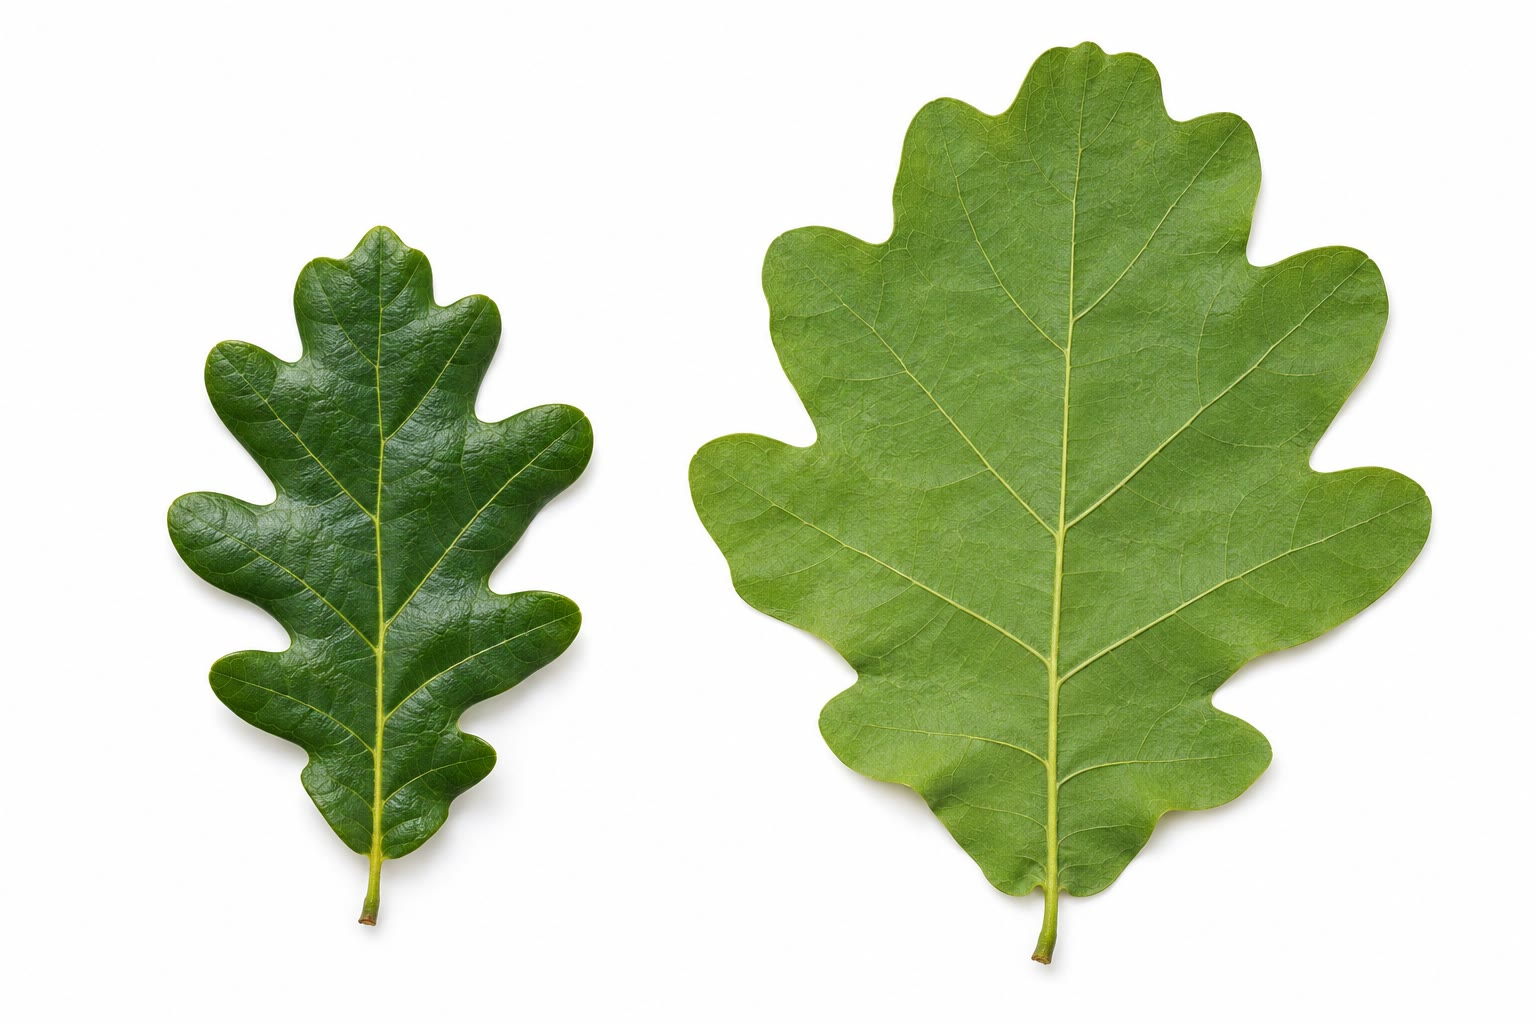
\includegraphics[width=0.55\linewidth]{images/book4/ai/b4-15-sun-shade-leaves.jpg}

{\small \omterm{prop:b2:plant-plasticity:sunshade}{ورقة شمس} \omterm{prop:b2:plant-plasticity:sunshade}{وورقة ظل} من بلوطة واحدة: \omterm{def:b2:meiosis-heredity:vocabulary}{النمط الوراثي} نفسه،
وضوء مختلف، وورقتان مختلفتان.}
\end{omfigure}

\section{قراءة الضوء}

\begin{theorem}[الفيتوكروم مقياسًا لنوعية الضوء]\label{thm:b2:plant-plasticity:phytochrome}
\index{فيتوكروم}\index{نسبة الأحمر إلى الأحمر البعيد}\index{تجنب الظل}
يوجد الفيتوكروم في صورتين: $P_r$ التي تمتص الضوء الأحمر
(\qty{660}{nm}) وتتحول إلى $P_{fr}$، و$P_{fr}$ التي
تمتص الأحمر البعيد (\qty{730}{nm}) وتتحول رجوعًا --- و
$P_{fr}$ هي الفعالة. وفي الضوء المستمر يتوازن التحولان
عند \emph{توازن ضوئي} يتوقف موضعه على \omterm{thm:b2:plant-plasticity:phytochrome}{نسبة
الأحمر إلى الأحمر البعيد} في الضوء وحدها:
\[
\varphi = \frac{P_{fr}}{P_{r} + P_{fr}} = \frac{R}{R + a\,FR},
\]
حيث $R$ و$FR$ كثافتا تدفق الفوتونات في النطاقين
و$a$ ثابت للصباغ ($a \approx 0.77$). ولضوء الشمس
$R{:}FR \approx 1.15$، فيعطي $\varphi \approx 0.6$؛ أما الضوء المرشَّح
عبر الأوراق، التي تمتص الأحمر وتمرر الأحمر البعيد، فله $R{:}FR
\approx 0.2$ و$\varphi \approx 0.2$. والقيمة $\varphi$ المنخفضة تقول للنبات
إنه تحت نباتات أخرى أو بجانبها قبل أن يكون مظللًا
فعلًا --- إذ يُكشف الأحمر البعيد المنعكس عن جار على
الجانب المواجه له --- فيستجيب \emph{بمتلازمة \omterm{thm:b2:plant-plasticity:phytochrome}{تجنب
الظل}}: استطالة ساق أسرع، وأعناق أطول، وأوراق مرفوعة
صاعدة، وتفرع أقل، وإزهار أبكر. والبادرة في مظلة مغلقة
تضاعف معدل استطالتها.
\end{theorem}
\begin{proof}
ليكن $k_1 R$ ثابت معدل التحول $P_r \to P_{fr}$ (وهو يتناسب
مع التدفق الأحمر) و$k_2\,FR$ ثابت التحول $P_{fr} \to P_r$. وعند
التوازن يكون $k_1 R\,P_r = k_2\,FR\,P_{fr}$، ومنه $P_{fr}/P_r = k_1 R/
(k_2 FR)$ و$\varphi = P_{fr}/(P_r + P_{fr}) = R/(R + a\,FR)$ مع
$a = k_2/k_1$. (وتمتص الصورتان قليلًا في النطاقين معًا، وهو ما
يستوعبه الثابت $a$؛ وشكل النتيجة لا يتغير.) فمع
$a = 0.77$: $1.15/(1.15 + 0.77) = 0.60$؛ و$0.2/(0.2 + 0.77) = 0.21$.
\end{proof}

\begin{omfigure}
\begin{tikzpicture}
\begin{axis}[
  width=0.7\linewidth, height=5.2cm,
  axis x line=bottom, axis y line=left,
  xmin=0, xmax=1.4, ymin=0, ymax=0.8,
  xlabel={نسبة الأحمر إلى الأحمر البعيد في الضوء}, ylabel={$\varphi = P_{fr}/P_{\text{الكلي}}$},
  xlabel style={font=\small, at={(axis description cs:0.5,-0.13)}, anchor=north},
  ylabel style={font=\small},
  tick label style={font=\small}, xtick={0,0.2,0.6,1.15}, ytick={0,0.2,0.4,0.6},
  clip=false,
]
\addplot[very thick, omDef, domain=0:1.4, samples=60] {x/(x+0.77)};
\draw[dashed, gray] (axis cs:1.15,0) -- (axis cs:1.15,0.6) -- (axis cs:0,0.6); \node[font=\scriptsize, anchor=south west] at (axis cs:1.15,0.6) {شمس مكشوفة};
\draw[dashed, gray] (axis cs:0.2,0) -- (axis cs:0.2,0.21) -- (axis cs:0,0.21); \node[font=\scriptsize, anchor=west] at (axis cs:0.25,0.15) {تحت مظلة};
\end{axis}
\end{tikzpicture}

{\small التوازن الضوئي للفيتوكروم بدلالة \omterm{thm:b2:plant-plasticity:phytochrome}{نسبة الأحمر إلى الأحمر
البعيد}. ضوء الشمس يبقي معظم الصباغ في الصورة الفعالة؛
والضوء المرشَّح بالأوراق يبقيه خاملًا في معظمه، ويقرأ النبات
الفرق جيرانًا.}
\end{omfigure}

\begin{proposition}[الانتحاء الضوئي]\label{prop:b2:plant-plasticity:phototropism}
\index{انتحاء ضوئي}\index{انتحاء}\index{فرضية خولودني--فينت}
\emph{الانتحاء} حركة نمو يوجهها منبه
اتجاهي. وفي \emph{\omterm{prop:b2:plant-plasticity:phototropism}{الانتحاء الضوئي}} ينحني الفرع نحو الضوء الأزرق:
إذ يُستشعر الضوء عند القمة بمستقبل للضوء الأزرق
(الفوتوتروبين)، ويُعاد توجيه الأوكسين النازل من القمة
نحو الجانب المظلل --- إذ تنتقل ناقلاته إلى الغشاء الجانبي
--- فيستطيل الجانب المظلل، وقد تلقى أوكسينًا أكثر، أسرع
من الجانب المضاء، فينحني الفرع نحو الضوء. و
الانحناء نمو تفاضلي لا عضلة: فهو لا يقع إلا في
\omterm{prop:b2:plant-meristems:ram}{منطقة الاستطالة}، ويستغرق ساعة أو ساعتين، وهو لاعكوس.
أما الجذور، التي \emph{يثبّط} فيها فائض الأوكسين نفسه الاستطالة،
فتنحني بعيدًا.
\end{proposition}
\begin{proof}[شواهد]
بيّن داروين (1880) بأغماد سويقات النجيليات أن القمة تدرك
الضوء وأن المنطقة تحتها تنحني: فتغطية القمة بغطاء
معتم ألغى الانحناء، وتغطية القاعدة بأنبوب لم
تلغه، والغطاء الشفاف تركه سليمًا. وقطع بويسن-ينسن (1913)
القمة ووضع مكانها كتلة من الجيلاتين بينهما: فبقي الانحناء،
إذن الإشارة مادة قابلة للانتشار؛ وصفيحة من الميكا
مقحمة في الجانب المظلل سدّتها، وفي الجانب المضاء لم تسدّها، إذن
المادة تسافر نزولًا في الجانب المظلل. وجمع فينت (1928)
المادة في آغار من قمم مقطوعة فوجد أن كتلة موضوعة
في غير المركز على غمد سويقة مقطوع الرأس في الظلام تجعله ينحني
بعيدًا عن الكتلة --- بزاوية تتناسب مع المقدار ---
وبجمع آغار من نصفي قمة مضاءة من جانب واحد،
وجد نحو ثلثي الأوكسين في الجانب المظلل وثلثه
في الجانب المضاء (بريغز، 1957، بطرائق أفضل). وإعادة
التوزيع الجانبية لهرمون نمو هي \omterm{prop:b2:plant-plasticity:phototropism}{فرضية خولودني--فينت}،
وقد صمدت.
\end{proof}

\begin{omfigure}
\begin{tikzpicture}[every node/.style={font=\scriptsize}, >=stealth]
  \foreach \x/\lab/\cap/\bend in {0/{سليم:\\ينحني}/0/1, 2.6/{القمة مغطاة:\\لا انحناء}/1/0, 5.2/{القاعدة مغطاة:\\ينحني}/2/1, 7.8/{القمة مقطوعة:\\لا انحناء}/3/0, 10.4/{القمة على جيلاتين:\\ينحني}/4/1} {
    \begin{scope}[xshift=\x cm]
      \fill[omExo!30] (-0.7,0) rectangle (0.7,0.2);
      \ifnum\bend=1
        \draw[very thick, omExo!70!black] (0,0.2) -- (0,1.6) .. controls (0,2.3) and (0.5,2.6) .. (0.9,2.8);
      \else
        \draw[very thick, omExo!70!black] (0,0.2) -- (0,3.0);
      \fi
      \ifnum\cap=1 \fill[black] (-0.2,2.7) rectangle (0.2,3.1); \fi
      \ifnum\cap=2 \fill[black] (-0.2,0.2) rectangle (0.2,1.5); \fi
      \ifnum\cap=3 \draw[thick] (-0.3,2.6) -- (0.3,2.6); \fi
      \ifnum\cap=4 \fill[omDef!35] (-0.2,2.55) rectangle (0.2,2.75); \draw[very thick, omExo!70!black] (0.55,2.75) -- (0.9,3.1); \fi
      \node[below, align=center] at (0,-0.15) {\lab};
    \end{scope}
  }
  \node[anchor=east, align=right, omProp!80!black] at (-1.0,2.2) {ضوء من\\اليمين $\to$};
\end{tikzpicture}

{\small تجارب غمد السويقة. داروين: القمة تستشعر
الضوء والمنطقة تحتها تنحني؛ وتغطية القمة توقف ذلك،
وحجب القاعدة لا يوقفه. وبويسن-ينسن: الإشارة تعبر
كتلة من الجيلاتين --- فهي مادة.}
\end{omfigure}

\begin{omfigure}
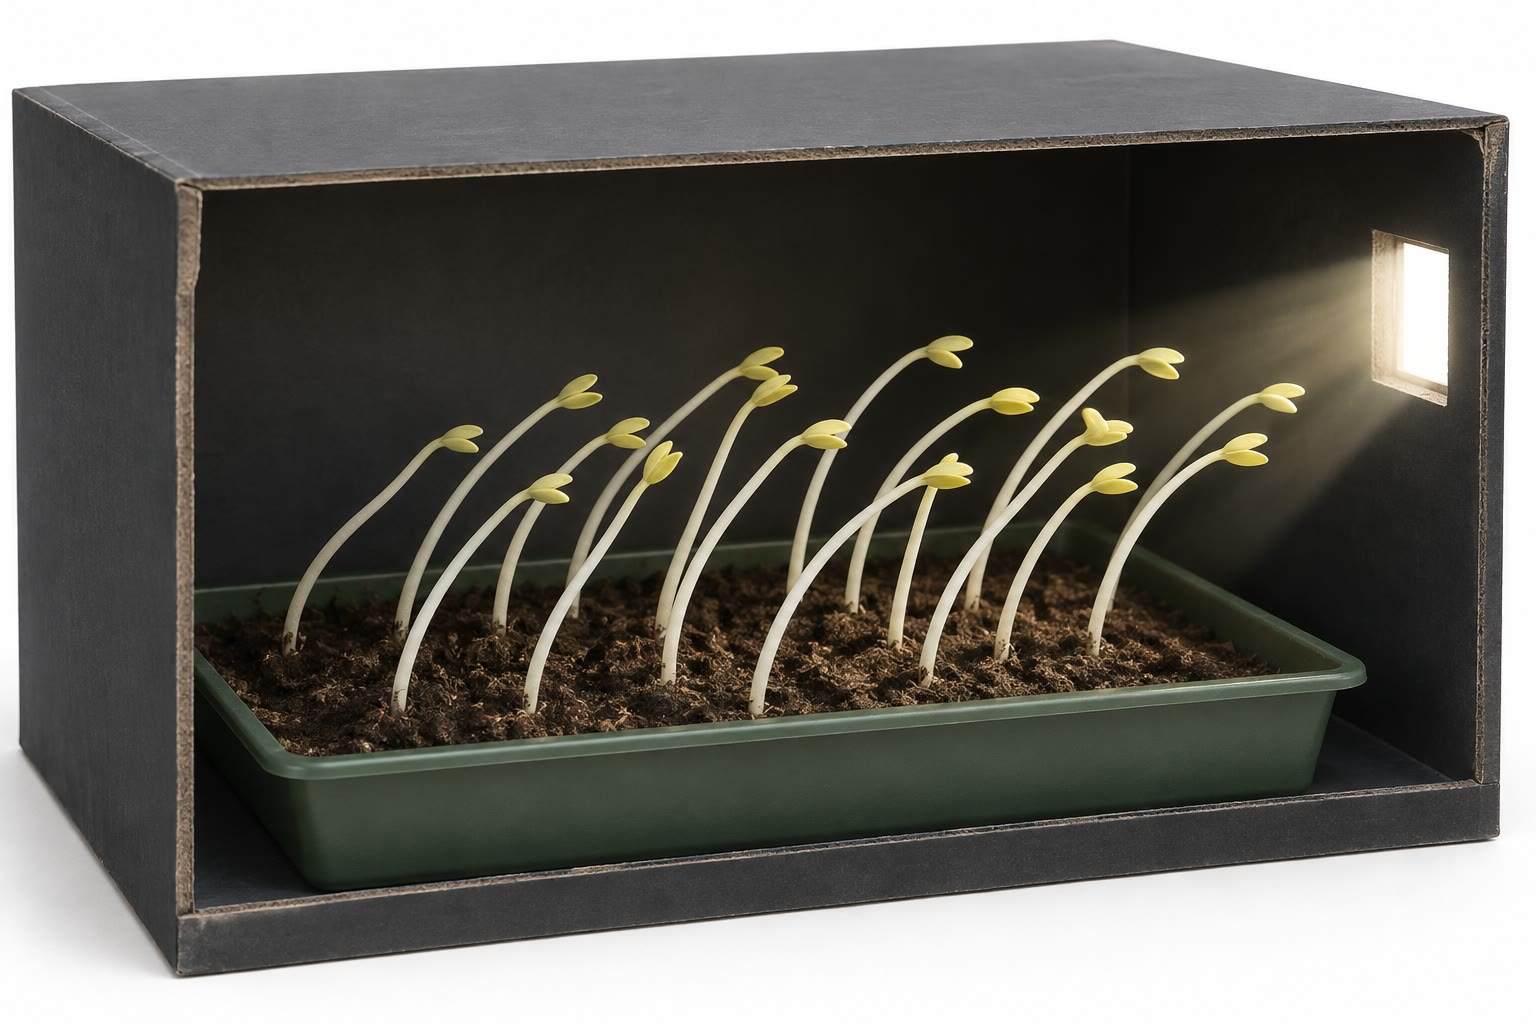
\includegraphics[width=0.55\linewidth]{images/book4/ai/b4-15-phototropism.jpg}

{\small بادرات في صندوق ذي نافذة واحدة: كلها تنحني نحو
الضوء، بنموها أسرع في الجانب البعيد عنه.}
\end{omfigure}

\begin{theorem}[كم تنحني ساق]\label{thm:b2:plant-plasticity:bend}
إذا استطال الجانب المظلل من ساق قطرها $d$ بمقدار نسبي
$\varepsilon_s$ واستطال الجانب المضاء بمقدار $\varepsilon_l$ على
منطقة نمو طولها $L$، انحنت المنطقة بزاوية
\[
\theta = \frac{L\,(\varepsilon_s - \varepsilon_l)}{d}
\]
(بالراديان). فغمد سويقة ينمو \qty{5}{\%} في الساعة على
منطقة من \qty{10}{mm} وعرضه \qty{1}{mm}، مع انقسام الأوكسين
$65 : 35$ بحيث ينمو الجانبان بمعاملي $1.3$ و$0.7$ من
المتوسط، ينحني في ثلاث ساعات بمقدار $\theta = 10\times(0.195 - 0.105)/1 =
0.9$ راديان، أي نحو \qty{50}{\degree}. والانحناء لا يحتاج إلى آلية
جديدة: فالنمو العادي في \cref{ch:b2:plant-meristems}، مجعولًا
غير متساوٍ على جانبين، يكفي.
\end{theorem}
\begin{proof}
يصير جانبا المنطقة قوسين نصفا قطريهما $\rho + d/2$ و
$\rho - d/2$ يقابلان الزاوية $\theta$ نفسها، وطولاهما $L(1 +
\varepsilon_s)$ و$L(1 + \varepsilon_l)$؛ وفرقهما
$\theta d$، ومنه $\theta = L(\varepsilon_s - \varepsilon_l)/d$. وعلى مدى
ثلاث ساعات عند \qty{5}{\%} في الساعة يكون متوسط الاستطالة $0.15$؛
و$1.3\times 0.15 = 0.195$ و$0.7\times 0.15 = 0.105$.
\end{proof}

\begin{proposition}[الانتحاء الأرضي]\label{prop:b2:plant-plasticity:gravitropism}
\index{انتحاء أرضي}\index{حصاة توازن}
الفرع الموضوع على جنبه يتجه صاعدًا والجذر نازلًا في غضون
ساعات. ويُستشعر اتجاه الجاذبية بواسطة \emph{حصى التوازن} ---
وهي حبيبات نشاء كثيفة في خلايا متخصصة من \omterm{prop:b2:plant-meristems:ram}{قلنسوة الجذر} ومن
غمد نشاء الساق --- تستقر إلى الجانب السفلي من الخلية
في ثوان، وتعيد، بضغطها على الغشاء أو على الشبكة
الهيولية الباطنة، توجيه ناقلات الأوكسين فيتراكم الأوكسين
في الجانب السفلي. وفي الفرع ينمو الجانب السفلي أسرع و
تنحني الساق صاعدة؛ وفي الجذر يثبّط فائض الأوكسين نفسه الجانب
السفلي، فينمو الجانب العلوي أسرع، وينحني الجذر نازلًا. وانزع
\omterm{prop:b2:plant-meristems:ram}{قلنسوة الجذر} ينمُ الجذر مستقيمًا في أي اتجاه؛ والطافرات الخالية
من النشاء تستشعر الجاذبية بضعف؛ والجذر على أسطوانة دوّارة ببطء
(كلينوستات)، لا تدع حصى التوازن تستقر أبدًا، ينمو
بلا اتجاه. والاستجابة استعمال ثانٍ لآلية
خولودني--فينت، بمستشعر مختلف.
\end{proposition}

\section{الماء: إغلاق المسام}

\begin{proposition}[التحكم في الثغور]\label{prop:b2:plant-plasticity:stomata}
\index{ثغر}\index{خلية حارسة}\index{حمض الأبسيسيك}\index{الناقلية الثغرية}
مسام الورقة، أي \emph{الثغور}، يحد كلًا منها
\emph{خليتان حارستان} جدراهما مثخنان على نحو غير متساوٍ، فحين
تأخذان البوتاسيوم والماء وتنتفخان تتقوسان متباعدتين فتفتحان
المسمّ، وحين تفقدانهما تغلقانه. وهي تنفتح في
الصباح تحت الضوء الأزرق و$\mathrm{CO_2}$ الداخلي المنخفض، و
تنغلق في الظلام؛ وتنغلق في دقائق حين يصل \emph{\omterm{def:b2:plant-flowering:dormancy}{حمض
الأبسيسيك}} --- المصنوع في جذور تستشعر تربةً تجف والمحمول
صعودًا في \omterm{def:b2:plant-meristems:wood}{الخشب}، أو المصنوع في الورقة نفسها وهي تفقد امتلاءها ---
وحين يكون الهواء شديد الجفاف. و\emph{\omterm{prop:b2:plant-plasticity:stomata}{الناقلية الثغرية}} $g_s$
تضبط الماء المفقود، $E = g_s\,(w_i - w_a)$ (وهو فرق
الكسر المولي لبخار الماء بين داخل الورقة، المشبع، و
الهواء)، وتضبط $\mathrm{CO_2}$ المأخوذ، $A = g_s\,(c_a -
c_i)/1.6$ (والعامل $1.6$ نسبة انتشاريتي
بخار الماء و$\mathrm{CO_2}$). فالورقة تبادل الماء بالكربون
عبر صمام واحد، و\emph{كفاءة استعمالها للماء} هي
\[
\frac{A}{E} = \frac{c_a - c_i}{1.6\,(w_i - w_a)},
\]
أي بضعة أجزاء من ألف من المول من الكربون لكل مول من الماء: فالورقة
C$_3$ النموذجية تنفق \qtyrange{400}{600}{g} من الماء لكل غرام كربون
مثبَّت، والورقة C$_4$ نصف ذلك، \omterm{prop:b2:plant-plasticity:xerophytes}{ونبات CAM} خمسه.
\end{proposition}

\begin{omfigure}
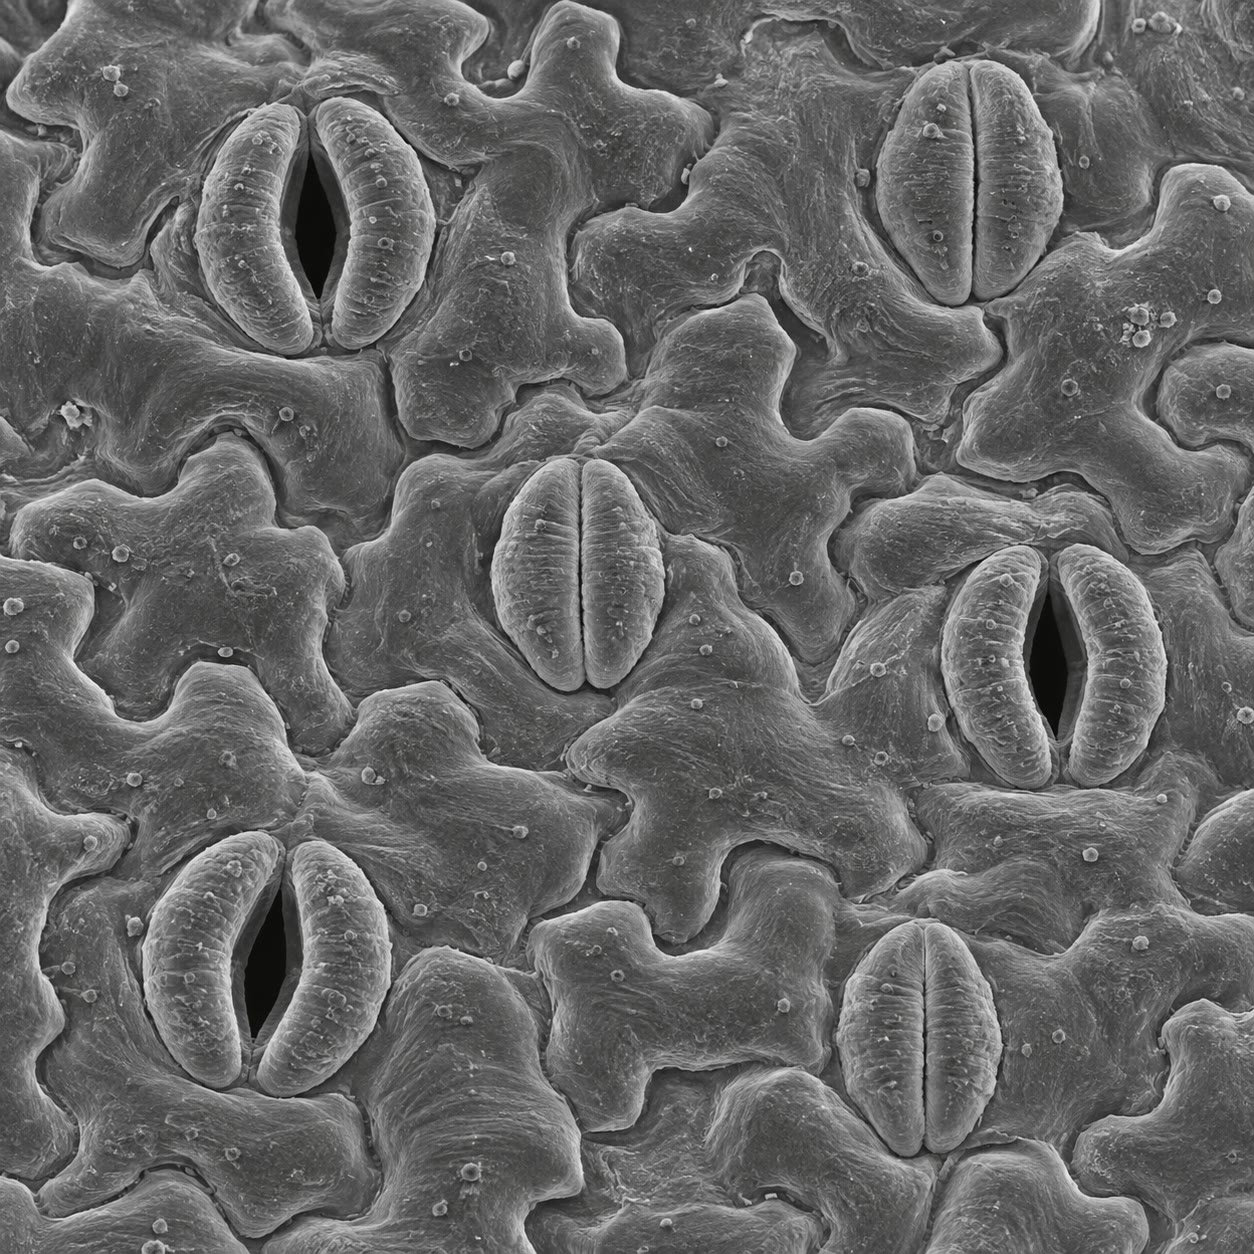
\includegraphics[width=0.42\linewidth]{images/book4/ai/b4-15-stomata-sem.jpg}

{\small ثغور على الوجه السفلي لورقة، بعضها مفتوح وبعضها
مغلق: خليتان حارستان حول كل مسمّ، وهو الصمام الذي
تبادل الورقة عبره الماء بثاني أكسيد الكربون.}
\end{omfigure}

\begin{example}[كلفة كربون يوم واحد]\label{ex:b2:plant-plasticity:wue}
عند الظهيرة تنتح ورقة عباد شمس لها $g_s = \qty{0.3}{mol.m^{-2}.s^{-1}}$،
و$w_i - w_a = 0.02$، و$c_a - c_i = \qty{120}{\micro mol/mol}$
مقدار $E = \qty{6}{mmol.m^{-2}.s^{-1}}$ وتثبّت $A =
0.3\times 120/1.6 = \qty{22}{\micro mol.m^{-2}.s^{-1}}$: ومنه $A/E =
\qty{3.7e-3}{}$، أي 270 جزيء ماء لكل ذرة كربون،
أي \qty{400}{g} من الماء لكل غرام كربون. وهكتار من أوراق كهذه
يفقد \qty{40}{t} من الماء في يوم صيفي ليثبّت \qty{100}{kg} من
الكربون. وحين تجف التربة، يغلق \omterm{def:b2:plant-flowering:dormancy}{حمض الأبسيسيك} الثغور إلى
عُشر هذه الناقلية: فيهبط $E$ عشرة أضعاف، ويهبط $A$ أقل من ذلك
(إذ يهبط $c_i$ أيضًا)، وينجو النبات على حمية
تجويع بدل أن يموت عطشًا.
\end{example}

\begin{proposition}[التكيفات مع الجفاف]\label{prop:b2:plant-plasticity:xerophytes}
\index{نبات جفافي}\index{نبات CAM}\index{عصاري}
تجمع نباتات الأماكن الجافة (\emph{الجفافيات}) بين بنى
موروثة واستراتيجيات. فلتقليل الفقد: بشرة سميكة، وثغور
غائرة في حفر أو تحت أشعار (تثخّن طبقة الهواء الساكن)،
وأوراق مختزلة إلى أشواك (الصبار) أو مطروحة في الموسم الجاف، وأوراق
صغيرة سميكة تتدحرج. وللتخزين: سوق وأوراق عصارية بمخاط
حابس للماء. وللبلوغ: جذور بعمق \qty{50}{m} (المسكيت) أو
منتشرة تحت السطح مباشرة لالتقاط زخة. وللتحويل: نباتات CAM
تفتح ثغورها ليلًا، حين يكون $w_i - w_a$ صغيرًا، وتثبّت
$\mathrm{CO_2}$ في حمض الماليك، وتعيد تثبيته خلف ثغور مغلقة
نهارًا --- أي الكربون نفسه بخمس الماء. وللهرب: حوليات الصحراء
تعيش بذورًا سنوات وتتم \omterm{def:b2:plant-life-cycles:cycles}{دورة حياة} في
الأسابيع التالية للمطر. وللاحتمال: نباتات البعث تفقد \qty{95}{\%} من
مائها وتحيا من جديد. ولكل استراتيجية ثمن --- فنمط CAM بطيء،
والعصارية ثقيلة، والأشواك لا تركّب ضوئيًا --- و
النبات الذي يدفعه يُغلب حيث يكثر الماء.
\end{proposition}

\begin{omfigure}
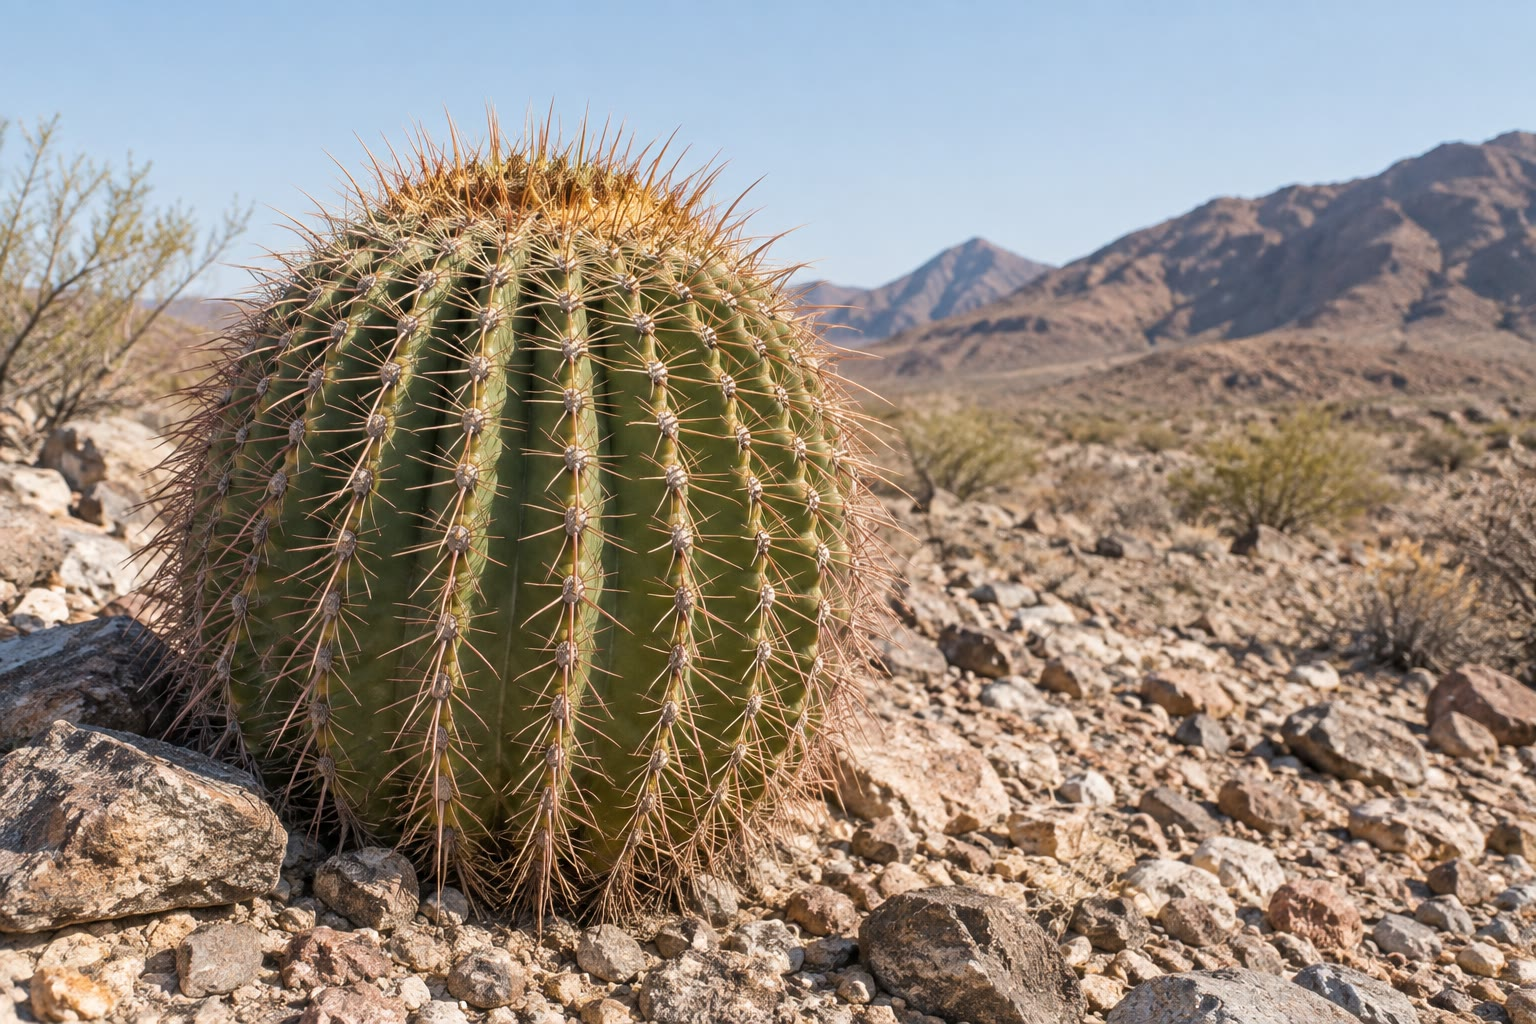
\includegraphics[width=0.55\linewidth]{images/book4/ai/b4-15-cactus.jpg}

{\small صبار برميلي: ساق عصارية ببشرة سميكة، و
أضلاع تدعه ينتفخ بعد المطر، وأوراق مختزلة إلى أشواك، و
ثغور لا تفتح إلا ليلًا.}
\end{omfigure}

\section{البرد والملح واستجابة الإجهاد}

\begin{proposition}[التأقلم مع الإجهاد]\label{prop:b2:plant-plasticity:stress}
\index{تأقلم بارد}\index{نبات ملحي}\index{بروتين الصدمة الحرارية}
أسبوع عند \qty{4}{\celsius} يخفض الحرارة التي تقتل
جاودار الشتاء من \qty{-5}{\celsius} إلى \qty{-25}{\celsius}: إذ
تكون الخلايا قد حمّلت سكريات وبروتينات تخفض نقطة التجمد
وتحمي الأغشية، وغيّرت شحومها لتبقى سيّالة، وصنعت
بروتينات مانعة للتجمد توقف نمو بلورات الثلج؛ والحدث القاتل
ليس الثلج، الذي يتكون بلا ضرر بين الخلايا، بل
تجفاف الخلية إذ يغادرها الماء لينضم إلى الثلج. وبضع
ساعات عند \qty{40}{\celsius} تستحث \emph{بروتينات الصدمة الحرارية} التي
تعيد طي البروتينات المتمسخة وتحمي الخلية عند
\qty{45}{\celsius}. أما الملح فيُلقى بالإقصاء عند الجذر، و
بالحجز في الفجوة (مع منحلّات متوافقة في
السيتوسول لتوازنه)، وفي \emph{النباتات الملحية} الحقيقية، بالإفراز
عبر غدد ملحية. ومعظم هذه الاستجابات يمر بالإشارات
نفسها: مستشعر، وارتفاع كالسيوم السيتوسول، \omterm{def:b2:plant-flowering:dormancy}{وحمض الأبسيسيك}،
وطائفة من \omterm{prop:b2:cell-differentiation:transcriptional}{عوامل الاستنساخ} تشعل مئات
المورّثات الواقية --- أي برنامج إجهاد عام كعموم المناعة
عند حيوان، ومكلف مثله: فالنبات المتأقلم
ينمو ببطء، والنبات الذي يتأقلم حين لا يحتاج يُغلب أمام
الذي لا يتأقلم.
\end{proposition}
\begin{proof}[شواهد]
تقيس تجارب \omterm{prop:b2:plant-plasticity:stress}{التأقلم البارد} الحرارة التي يموت عندها نصف
خلايا ورقة (وهي LT$_{50}$) قبل فترة من الحرارة
المنخفضة وبعدها؛ والانزياح، وهو من عشر درجات إلى عشرين في أسبوع،
يُعكس بأسبوع من الدفء. والطافرات العاجزة عن إشعال برنامج
البرد (\omterm{prop:b2:cell-differentiation:transcriptional}{عوامل الاستنساخ} CBF) تتأقلم بضعف، و
النباتات المعبّرة عن تلك العوامل باستمرار تنجو من الصقيع
بلا \omterm{def:b2:plant-plasticity:plasticity}{تأقلم} --- لكنها تنمو أقزامًا.
\end{proof}

\begin{omfigure}
\begin{tikzpicture}[every node/.style={font=\scriptsize}, >=stealth]
  \node[draw, rounded corners, fill=omExo!25, align=center] (s) at (0,0) {إجهاد\\جفاف، أو برد،\\أو ملح، أو حرارة};
  \node[draw, rounded corners, fill=omDef!15, align=center] (sen) at (3.2,0) {مستشعر\\(غشاء، أو امتلاء،\\أو بروتينات غير مطوية)};
  \node[draw, rounded corners, fill=omDef!15, align=center] (ca) at (6.4,0) {رسل ثوانٍ\\Ca$^{2+}$، وABA};
  \node[draw, rounded corners, fill=omProp!20, align=center] (tf) at (9.6,0) {عوامل\\استنساخ};
  \node[draw, rounded corners, fill=omThm!15, align=center] (out) at (12.8,0.9) {مورّثات واقية:\\منحلّات، ومانعات تجمد،\\ومرافقات، وناقلات};
  \node[draw, rounded corners, fill=omThm!15, align=center] (out2) at (12.8,-0.9) {نمو أبطأ:\\وهو الثمن};
  \draw[->, thick] (s) -- (sen); \draw[->, thick] (sen) -- (ca); \draw[->, thick] (ca) -- (tf);
  \draw[->, thick] (tf) -- (out); \draw[->, thick] (tf) -- (out2);
\end{tikzpicture}

{\small الشكل المشترك لاستجابة النبات للإجهاد: مستشعر، وإشارة
كالسيوم وحمض أبسيسيك، \omterm{prop:b2:cell-differentiation:transcriptional}{وعوامل استنساخ}، و
برنامج من المورّثات الواقية --- مدفوع من النمو.}
\end{omfigure}

\begin{example}[إشارات تكذب]\label{ex:b2:plant-plasticity:lie}
اللدونة لا تزيد جودةً على الإشارة. فالبادرة تحت ظل جار
أحمر بعيد تستطيل --- وهي محقة إن كان الجار بادرة
تستطيع أن تعلوها؛ وهي هالكة إن كان شجرة، إذ تضيع المدخرات
المنفقة على الساق على الجذر والورقة. والمحاصيل المزروعة كثيفة تظلل
بعضها بعضًا، فتستطيل وترقد؛ وقد انتخب المربّون أقماحًا وأرزًا
يتجاهلان إشارة الأحمر البعيد. وأسبوع دافئ في شباط يخرج
أوراقًا يقتلها صقيع آذار؛ والنباتات التي تنجو هي التي
تعدّ البرد أيضًا (\cref{ch:b2:plant-flowering}). فكل
استجابة لدنة رهان على صدق الإشارة، \omterm{def:b2:plant-plasticity:plasticity}{ومعيار
الاستجابة} يشكّله كم مرة، في ماضي السلالة، قالت الإشارة
الحقيقة.
\end{example}

\section{تمارين}

\begin{exercise}[$\star$]\label{exo:b2:plant-plasticity:1}
عرّف \omterm{def:b2:plant-plasticity:plasticity}{اللدونة النمطية} \omterm{def:b2:plant-plasticity:plasticity}{ومعيار الاستجابة} \omterm{def:b2:plant-plasticity:plasticity}{والتأقلم} و
\omterm{def:b2:plant-plasticity:plasticity}{التكيف}، مع مثال نباتي على كل منها.
\end{exercise}

\begin{exercise}[$\star$]\label{exo:b2:plant-plasticity:2}
صف معالجات داروين الأربع لغمد السويقة وما بيّنته كل منها.
\end{exercise}

\begin{exercise}[$\star$]\label{exo:b2:plant-plasticity:3}
اذكر خمسة فروق بين \omterm{prop:b2:plant-plasticity:sunshade}{ورقة شمس} \omterm{prop:b2:plant-plasticity:sunshade}{وورقة ظل}، وقل
متى في حياة الورقة يُتخذ الاختيار.
\end{exercise}

\begin{exercise}[$\star$]\label{exo:b2:plant-plasticity:4}
كيف ينفتح الثغر، وما الذي يفتحه في الصباح، وما الذي يغلقه
في جفاف؟
\end{exercise}

\begin{exercise}[$\star\star$]\label{exo:b2:plant-plasticity:5}
احسب $\varphi$ من أجل $R{:}FR = 1.15$ (شمس)، و$0.7$ (فرجة)، و$0.2$
(تحت مظلة) و$0.05$ (ظل عميق) مع $a = 0.77$. وبين
أي اثنين منها يشعل النبات \omterm{thm:b2:plant-plasticity:phytochrome}{تجنب الظل} إذا كانت
العتبة $\varphi = 0.4$؟
\end{exercise}

\begin{exercise}[$\star\star$]\label{exo:b2:plant-plasticity:6}
ورقة لها $g_s = \qty{0.25}{mol.m^{-2}.s^{-1}}$، و$w_i - w_a = 0.025$،
و$c_a - c_i = \qty{100}{\micro mol/mol}$. احسب $E$ و$A$، و
كفاءة استعمال الماء بالمولات وبغرامات الماء لكل غرام
كربون، والماء المفقود في المتر المربع في نهار من 12 ساعة.
\end{exercise}

\begin{exercise}[$\star\star$]\label{exo:b2:plant-plasticity:7}
أعد حساب التمرين السابق من أجل \omterm{prop:b2:plant-plasticity:xerophytes}{نبات CAM} تنفتح ثغوره
ليلًا مع $w_i - w_a = 0.005$ والناقلية نفسها. فبأي
عامل تنخفض كلفة الكربون من الماء؟
\end{exercise}

\begin{exercise}[$\star\star$]\label{exo:b2:plant-plasticity:8}
\omterm{prop:b2:plant-plasticity:gravitropism}{حصاة توازن} حبيبة نشاء نصف قطرها \qty{2}{\micro m} وكثافتها
\qty{1500}{kg/m^3} في سيتوبلازم كثافته \qty{1100}{kg/m^3} و
لزوجته \qty{0.01}{Pa.s}. احسب سرعة ترسيبها (بستوكس) و
الزمن اللازم لعبور خلية \qty{10}{\micro m}. ولماذا يلغي كلينوستات
يدور مرة في الدقيقة الانتحاءَ الأرضي؟
\end{exercise}

\begin{exercise}[$\star\star$]\label{exo:b2:plant-plasticity:9}
ساق عرضها \qty{2}{mm} تنمو \qty{2}{\%} في الساعة على
منطقة \qty{20}{mm}. وضوء من جانب واحد يقسم الأوكسين $60 : 40$.
فبأي زاوية انحنت بعد ساعتين؟ وبعد كم تصير
على \qty{90}{\degree} من اتجاهها الأصلي؟
\end{exercise}

\begin{exercise}[$\star\star\star$]\label{exo:b2:plant-plasticity:10}
بادرة لها \qty{50}{mg} من المدخرات تستطيل \qty{2}{cm}
في اليوم في المكشوف و\qty{4}{cm} في اليوم تحت مظلة، وتنفق
\qty{1}{mg} من المدخرات لكل سنتيمتر ساق زائد عما توفره
أوراقها. والمظلة على \qty{30}{cm} فوقها في حقل قراص
وعلى \qty{10}{m} في غابة. ففي أي الحالتين ينجح \omterm{thm:b2:plant-plasticity:phytochrome}{تجنب الظل}،
وماذا يحدث في الأخرى؟
\end{exercise}

\begin{exercise}[$\star\star\star$]\label{exo:b2:plant-plasticity:11}
اشرح لماذا يقتل التجمد الخلية بالتجفاف لا بالثلج،
وماذا يفعل أسبوع من البرد لمنع ذلك، ولماذا يكون النبات الذي
يعبّر عن برنامج البرد طوال السنة قزمًا.
\end{exercise}

\begin{exercise}[$\star\star\star$]\label{exo:b2:plant-plasticity:12}
«اللدونة رهان على صدق إشارة.» ناقش ذلك بإشارة
الأحمر البعيد، والأسبوع الدافئ في شباط، وتربية محاصيل
تتجاهل جيرانها.
\end{exercise}

\section{مسألة: بادرة تحت المظلة}

\begin{problem}[{مسألة نهاية الأسبوع --- مناخ الضوء عند بادرة،
واستطالتها، وميزان مائها، وانتحاءاتها محسوبةً من فيزياء
مستشعراتها، وتنتهي إلى حالة فيتوكرومها، وطولها بعد أسبوعين،
واستعمالها اليومي للماء}]
\label{pb:b2:plant-plasticity:1}
تنبت بادرة بتولا تحت مظلة تمرر
\qty{3}{\%} من ضوء الشمس وتخفض $R{:}FR$ من $1.15$ إلى $0.2$
($a = 0.77$). وفي الشمس الكاملة كانت لتستطيل \qty{1.5}{cm} في اليوم؛
وتحت المظلة يُضرب معدل استطالتها في $1 +
2(0.6 - \varphi)$. وساقها عرضها \qty{2}{mm} بمنطقة نمو
\qty{15}{mm}. والأوراق: \qty{20}{cm^2} جميعها؛ و$g_s =
\qty{0.2}{mol.m^{-2}.s^{-1}}$؛ و$w_i - w_a = 0.015$ في الظل، و
$0.03$ في فرجة؛ و$c_a - c_i = \qty{80}{\micro mol/mol}$؛ والنهار
يدوم \qty{14}{h}. وحصى التوازن: نصف القطر \qty{2.5}{\micro m}، والكثافة
\qty{1500}{kg/m^3}، في سيتوبلازم \qty{1100}{kg/m^3} و
\qty{0.01}{Pa.s}.

\medskip
\noindent\textbf{الجزء الأول --- الضوء.}
\begin{enumerate}
  \item احسب $\varphi$ في المكشوف وتحت المظلة.
  \item ماذا تستنتج البادرة من $\varphi$، وماذا كانت
        لتستنتج لو مررت المظلة \qty{3}{\%} من
        الضوء دون أن تغير لونه (أي قماش تظليل)؟
  \item احسب معدل الاستطالة تحت المظلة.
  \item كم يبلغ طول البادرة بعد 14 يومًا هناك، في مقابل
        شقيقة في المكشوف؟
  \item تنفتح فرجة على أحد الجانبين، فترفع $R{:}FR$ في ذلك الجانب إلى
        $0.8$. فما الاستجابتان التاليتان، وبأي مستقبلين
        ضوئيين؟
  \item لماذا تكون الأوراق النامية تحت المظلة أكبر و
        أرق، وماذا يحدث لها إذا قُطعت المظلة؟
\end{enumerate}

\medskip
\noindent\textbf{الجزء الثاني --- الانحناء نحو الفرجة.}
\begin{enumerate}[resume]
  \item ضوء الفرجة يقسم الأوكسين $65 : 35$ عبر
        الساق. ومع معدل الاستطالة تحت المظلة في السؤال 3، احسب
        الاستطالة النسبية لكل جانب من منطقة النمو في
        ساعة واحدة.
  \item احسب زاوية الانحناء بعد ساعة.
  \item بعد كم تشير الساق مباشرة إلى الفرجة، إذا كانت
        الفرجة على \qty{60}{\degree} من الشاقول؟
  \item الساق مائلة الآن. احسب سرعة ترسيب
        \omterm{prop:b2:plant-plasticity:gravitropism}{حصاة توازن} والزمن اللازم لعبور خلية \qty{12}{\micro m}.
  \item \omterm{prop:b2:plant-plasticity:gravitropism}{الانتحاء الأرضي} للفرع وانتحاؤه الضوئي متعارضان الآن.
        فأيهما يغلب في نبات متجنب للظل، ولماذا يكون ذلك
        تكيفيًا؟
  \item جذر البادرة نفسها أمالته حصاة \qty{45}{\degree}. تنبّأ
        باستجابته واشرح لماذا تكون معاكسة لاستجابة الفرع مع أن
        الآلية واحدة.
\end{enumerate}

\medskip
\noindent\textbf{الجزء الثالث --- الماء.}
\begin{enumerate}[resume]
  \item احسب معدل النتح في المتر المربع في الظل،
        والماء الذي تفقده أوراق البادرة في اليوم.
  \item احسب الكربون المثبَّت في المتر المربع في الثانية وفي
        اليوم، وكفاءة استعمال الماء بغرامات الماء لكل غرام كربون.
  \item ما مجمل كسب البادرة اليومي من الكربون في الظل،
        بالمليغرامات؟
  \item أعد حساب الماء المفقود والكفاءة في الفرجة.
  \item تجف التربة ويخفض \omterm{def:b2:plant-flowering:dormancy}{حمض الأبسيسيك} $g_s$ إلى
        \qty{0.02}{mol.m^{-2}.s^{-1}}. أعد حساب $E$ و$A$
        (وافترض أن $c_a - c_i$ يرتفع إلى \qty{200}{\micro mol/mol}).
        فأيهما يهبط أكثر، ولماذا؟
  \item للبادرة \qty{5}{g} من نسيج الورق \qty{85}{\%} منه
        ماء وتستطيع فقد خمسه قبل الذبول. فكم تدوم
        في الفرجة والثغور مفتوحة إذا لم توفّر الجذور شيئًا؟
  \item اشرح لماذا لا تلائم استراتيجية CAM بادرة بتولا
        تحت مظلة.
\end{enumerate}

\medskip
\noindent\textbf{الجزء الرابع --- الرهان.}
\begin{enumerate}[resume]
  \item تحمل البادرة \qty{100}{mg} من المدخرات وتنفق
        \qty{2}{mg} لكل سنتيمتر ساق زائد عما توفره
        أوراقها في الظل. فكم ساقًا تستطيع بناءها بالمدخرات
        وحدها؟
  \item المظلة حقل قراص على \qty{40}{cm} فوقها؛ ثم غابة
        على \qty{8}{m} فوقها. قل في كل حالة هل تبلغ الاستطالة
        الضوء قبل أن تنفد المدخرات، وما كانت الاستجابة
        الأفضل في الغابة.
  \item البتولا رائدة الأرض المكشوفة؛ وبادرة الزان تستطيع
        الانتظار عقودًا في ظل عميق. قارن معياري استجابتهما
        المنتظرين للقيمة $\varphi$.
  \item يريد مربٍّ محصولًا مزروعًا كثيفًا لا يستطيل. فأي
        مستشعر أو استجابة تعطّل، وأي أثر جانبي يجب أن تتحقق منه؟
  \item اشرح في جملتين لماذا يكون النبات الذي لا يستطيع استشعار
        جيرانه والنبات الذي يصدّقهم دائمًا كلاهما أسوأ حالًا من
        الذي يصدّقهم أحيانًا.
  \item اذكر النتيجة: $\varphi$ في الشمس والظل، وطول
        البادرة بعد 14 يومًا، واستعمالها اليومي للماء في الظل
        وفي الفرجة.
\end{enumerate}
\end{problem}
